\documentclass[crop,tikz]{standalone}% 'crop' is the default for v1.0, before it was 'preview'
% \usetikzlibrary{...}% tikz package already loaded by 'tikz' option
\usepackage{tikz}
\usepackage{amsmath, amsthm, amssymb, amsfonts}
\usetikzlibrary{shapes,arrows.meta}
\usepackage{newtxtext,newtxmath,courier}
\DeclareMathAlphabet{\mathcal}{OMS}{cmsy}{m}{n}

% Talon's custom commands
\newcommand{\argmin}{\arg\!\min}
\newcommand{\me}{\mathrm{e}}
\providecommand{\e}[1]{\ensuremath{\times 10^{#1}}} 
\providecommand{\mb}[1]{\mathbf{#1}}
\providecommand{\mf}[1]{\mathfrak{#1}}
\providecommand{\mc}[1]{\mathcal{#1}}
\providecommand{\ro}{\mathbf{\mathbf{r}}_o}
\providecommand{\so}{\mathbf{\hat{s}}_o}
\providecommand{\rp}{\mathbf{r}_p}
\providecommand{\rbm}[1]{r_b^{\text{m}}}
\providecommand{\rd}{\mathbf{r}_d}
\providecommand{\rdf}{\mathpzc{r}_d}
\providecommand{\mh}[1]{\mathbf{\hat{#1}}}
\providecommand{\mbb}[1]{\mathbb{#1}}
\providecommand{\bs}[1]{\boldsymbol{#1}}
\providecommand{\bv}{\bs{\nu}}
\providecommand{\bvp}{\bs{\tau}}
\providecommand{\bsh}[1]{\hat{\boldsymbol{#1}}}
\providecommand{\nan}{\left(\frac{\text{NA}}{n_o}\right)}
\providecommand{\lmsum}{\sum_{l=0}^\infty\sum_{m=-l}^{l}}
\providecommand{\intr}[1]{\int_{\mbb{R}^{#1}}}
\providecommand{\ints}[1]{\int_{\mbb{S}^{#1}}}
\DeclareFontFamily{OT1}{pzc}{}
\DeclareFontShape{OT1}{pzc}{m}{it}{<-> s * [1.10] pzcmi7t}{}
\DeclareMathAlphabet{\mathpzc}{OT1}{pzc}{m}{it}
\newcommand{\eqname}[1]{\tag*{#1}}
\newcommand*\widefbox[1]{\fbox{\hspace{1em}#1\hspace{1em}}}

\tikzstyle{block} = [draw, fill=white, rectangle, minimum height=3em, minimum width=5em, align=center]
\begin{document}
  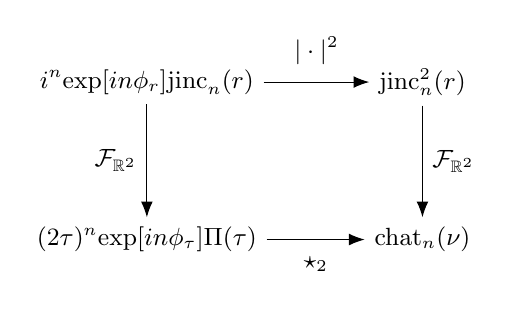
\begin{tikzpicture}[auto, node distance=2.5cm,>={Latex[length=2mm]}]
    \tikzset{font={\fontsize{9pt}{12}\selectfont}}
    \node [align=center] (sad) {$\text{jinc}_{n}^2(r)$};
    \node [left of=sad, node distance=3.5cm] (e) {$i^n\text{exp}[in\phi_r]\text{jinc}_{n}(r)$};
      \node [below of=sad, node distance=2.cm] (sds) {$\text{chat}_{n}(\nu)$};
        \node [left of=sds, node distance=3.5cm] (e2) {$(2\tau)^n\text{exp}[in\phi_\tau]\Pi(\tau)$};
      \draw [->] (e) -- node[shift={(0,0.1)}] {$|\cdot|^2$} (sad);
            \draw [->] (e2) -- node[below, shift={(0,-0.1)}] {$\star_2$} (sds);        
          \draw [->] (e) -- node[left] {$\mathcal{F}_{\mathbb{R}^2}$} (e2);
    \draw [->] (sad) -- node[right] {$\mathcal{F}_{\mathbb{R}^2}$} (sds);
      \end{tikzpicture}
\end{document}